\begin{frame}
	\frametitle{Estabilidad lineal por trayectorias}
	\begin{empheq}{equation*}
	dy(t)=\lambda y(t) dt +\beta dW_t, \qquad y_0=cte., \lambda, \beta \in \mathbb{R} \tag{E}.
	\end{empheq}
	\begin{columns}
		\column{.5\textwidth}
		\begin{overlayarea}{\textwidth}{.5\textheight}
			\centering Pullback attractor
			\only<2->{
				\begin{empheq}[box=\shadowbox*]{equation*}
				\lim_{t_0\to-\infty} y(t) =\widehat{O}_t %
				:= e^{\lambda t}\int\limits_{-\infty}^{t}e^{-\lambda s}dW_s, 
				\end{empheq}
			}
		\end{overlayarea}
		\column{.5\textwidth}
		\begin{overlayarea}{\textwidth}{.5\textheight}
			\vspace{-1.0cm}
			\only<3->{
				\begin{Teorema}
					Sea $\lambda<0$,  el método Steklov para (E)
					tiene el siguiente atractor
					\begin{equation*}
					\widehat{O}_n^{(h)}  :=
					\xi \sum_{j=-\infty}^{n-1}\exp(\lambda h(n-1-j)) \Delta B_j,
					\end{equation*}
					$\widehat{O}_n^{(h)} \to \widehat{O}_t$, \quad $h\to 0$, \quad pathwise.
				\end{Teorema}
			}
		\end{overlayarea}
	\end{columns}
	\begin{bibunit}[alpha]
		\nocite{Buckwar2011a}
		\biblio{BibliografiaTesis}
	\end{bibunit}		
\end{frame}
%%%%%%%%%%%%%%%%%%%%%%%%%%%%%%%%%%%%%%%%%%%%%%%%%%%%%%%%%%%%%%%%%%%%%%%%%%%%%%%%%%%%%%%%%%%%%%%%%
\begin{frame}
	\frametitle{Estabilidad en Media Cuadrática Ruido Multiplicativo}
	\begin{empheq}[box=\shadowbox*]{equation*}
	dy(t)=\lambda y(t) dt +\xi y(t) dW_t, \qquad y_0=cte., 
	\ \lambda, \xi \in \mathbb{R} \tag{E}.
	\end{empheq}
	\begin{columns}
		\column{.3\textwidth}
		\begin{overlayarea}{\textwidth}{\textheight}
			\only<2->{
				\begin{exampleblock}{MS-estabilidad Lineal}
					\begin{itemize}
						\item
						diagonal (EM)
						\item
						vertical (Steklov)
					\end{itemize}
				\end{exampleblock}
			}
		\end{overlayarea}
		\column{.7\textwidth}
		\begin{overlayarea}{\textwidth}{\textheight}
			\only<3->{
				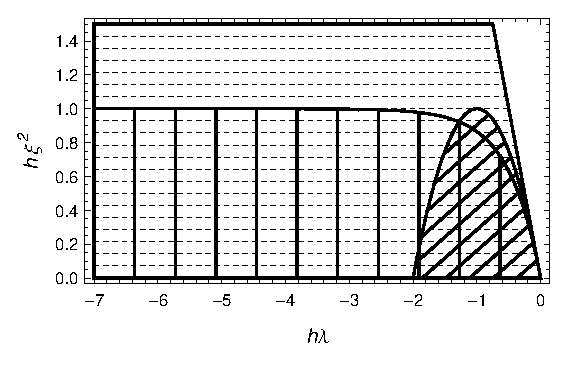
\includegraphics[width=1\linewidth]{images/StabilityPlotMultiplicativeNoise}
			}
		\end{overlayarea}
	\end{columns}
\end{frame}
